\documentclass[letterpaper, 12pt]{article}
\usepackage[francais]{babel}

\usepackage{amsmath,amsfonts,amsthm,amssymb, graphicx,wasysym,multirow}
\usepackage[latin1]{inputenc}

\pagestyle{plain}

\setlength{\topmargin}{-2cm}
\setlength{\textheight}{23.5cm}
\setlength{\textwidth}{18cm}
\setlength{\oddsidemargin}{-1cm}
\setlength{\parindent}{0pt}

%\pdfoutput=1


\begin{document}

611-- Which of the following four statements is true?\\

a) The total area ratio of two similar solids is half of the
similarity ratio of the two solids.\\
b) The total area ratio of two similar solids is equal to the similarity ratio
between two solids.\\
c) The total area ratio of two similar solids is equal to the square of the similarity
ratio between the two solids.\\
d) The total area ratio of two similar solids is equal to the cube of the similarity ratio between the two solids.\\

Answer: c)\\

Explanation: \\
The total area ratio of two similar solids is equal to the square of the similarity ratio between the two solids.
Thus, the answer is c).\\

621-- Among the four choices below, which one correctly completes the following statement: `` Two figures that have a similarity ratio of $\ldots$ are isometric."?\\
a) 0\\
b) 1\\
c) 2\\
d) 4\\

Answer: b) \\

Explanation: \\
Two figures that have a similarity ratio of 1 are isometric. The correct answer is b).\\

631-- In a population or a sample of a population, which quartile does the median represent?\\

a) First quartile\\
b) Second quartile\\
c) Third quartile\\
d) Fourth quartile\\

Answer: b)\\

Explanation: \\
The median represents the second quartile. The correct answer is  b).\\

641-- What is the distribution mode of 1, 9, 12, 6, 3, 1, 4, 10, 9, 2,
11, 4, 7, 9, 3, 6, 6, 5, 2, 2, 6, 4, 7, 6, 2?\\

Answer: 6\\

Explanation: \\
Start by putting data in order.\\
1, 1, 2, 2, 2, 2, 3, 3, 4, 4, 4, 5, 6, 6, 6, 6, 6, 7, 7, 9, 9, 9, 10, 11,
12\\
The distribution mode is the piece of data used with the highest number of occurrences. In this data set the number 6 is the most frequently occuring value. Thus, the mode is 6.\\

651-- What is the percentile rank of a piece of data that is $45\,\%$ superior to all data?\\

Answer: 55\\

Explanation: \\
If 45\,\% of all data is superior to this piece of data, then 55\,\% are smaller to or equal to this number. The percentile rank is a number that indicates the percentage of data smaller than or equal to the indicated data.  Thus, the correct answer is 55.\\

661-- Among the following four statements, which one is true?\\

a) The answer to $(-4)^{432}$ is negative.\\
b) The answer to $-4^{432}$ is negative.\\
c) The answer to $-(-4)^{432}$ is positive.\\
d) The answer to $(-4)^{433}$ is positive.\\

Answer: b)\\

Explanation: \\
The answer to $-4^{432}$ is negative since only the number 4 is raised to the $432^{th}$ power. Even if $4^{432}$ is positive, the negative sign located in front of the number makes the overall result negative.\\
The correct answer is b).\\

671-- Of the four following equalities, which one is true?\\

a) $\sqrt{a}\cdot\sqrt{b}=ab$\\
b) $\sqrt{a}\cdot\sqrt{b}=a\sqrt{b}$\\
c) $\sqrt{a}\cdot\sqrt{b}=b\sqrt{a}$\\
d) $\sqrt{a}\cdot\sqrt{b}=\sqrt{ab}$\\

Answer: d)\\

Explanation: \\
$\sqrt{a}\cdot\sqrt{b}=\sqrt{ab}$\\
The correct answer is d).\\

681-- Which of the following statements is true?\\

a) If the product of four factors is 0, then one these factors is 0.  \\
b) If the product of four factors is 0, then at least two of these factors are 0.  \\
c) If the product of four factors is 0, then at least three of these factors are 0.  \\
d) If the product of four factors is 0, then all of these factors must also be 0.\\

Answer: a)\\

Explanation: \\
If the product of four factors is zero, then at least one of these factors is zero.  \\
The correct answer is a).\\

691-- What value must $w$ have in order for $wx^{2}\,-\,24x\,+\,9$ to be a perfect square?\\

Answer: 16\\

Explanation: \\
$(4x\,-\,3)^{2}=16x^{2}\,-\,24x\,+\,9$\\
The correct answer is 16.\\

701-- Of the four choices below, which one represents $(f\,-\,g)(-4)$
if $f(x)=3x\,+\,4$ and $g(x)=x^{2}\,-\,2x\,+\,1$?\\

a) $-36$\\
b) $-33$\\
c) $-30$\\
d) $-27$\\

Answer: b)\\

Explanation: \\
\begin{eqnarray*}
f(x)&=&3x\,+\,4\\
g(x)&=&x^{2}\,-\,2x\,+\,1\\
f(x)\,-\,g(x)&=&3x\,+\,4\,-\,(x^{2}\,-\,2x\,+\,1)\\
&=&3x\,+\,4\,-\,x^{2}\,+\,2x\,-\,1\\
&=&-x^{2}\,+\,5x\,+\,3\\
(f\,-\,g)(-4)&=& - (-4)^{2}\,+\,5\times(-4)\,+\,3\\
&=&-16\,-\,20\,+\,3\\
&=&-33\\
\end{eqnarray*}
The correct answer is b).\\

711-- Among the four following choices, which one is the image of 4 subject to the function $f(x)=(x\,-\,5)(x\,+\,3)$?\\

a) $-63$\\
b) $-7$\\
c) 7\\
d) 63\\

Answer: b)\\

Explanation: \\
By replacing $x$ with 4 in the equation
$f(x)=(x\,-\,5)(x\,+\,3)$.\\
We obtain $f(4)=(4\,-\,5)(4\,+\,3)=(-1)(7)=-7$.\\
The correct answer is b).\\

721-- Among the four following choices, which one represents the interval where the function $f(x)=2x\,+\,7$ is decreasing?\\

a) $\varnothing$\\
b) $]-\infty,0]$\\
c) $[0,\infty[$\\
d) $]-\infty,\infty[$\\

Answer: a)\\

Explanation: \\
The function $f(x)=2x\,+\,7$ represents a straight line with a positive slope. It is a strictly increasing function on the whole real line.
Therefore, there exists no nonempty interval where it is decreasing. The correct answer is a).
Here is a plot of $f(x)$.\\
    \begin{center}
    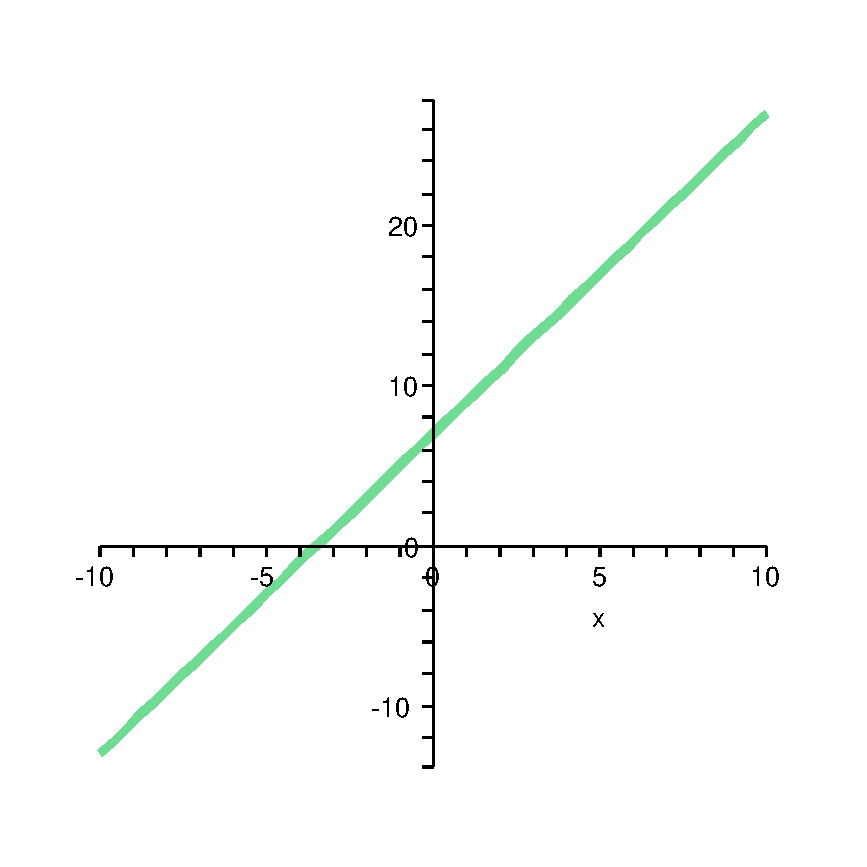
\includegraphics[width=6cm,bb=0 0 400 400]{fonction26.eps}
% fonction26.eps : 300dpi, width=3.39cm, height=3.39cm, bb=0 0 400 400
    \end{center}

731-- Among the four following statements, which one is true if the function $f(x)=ax^{2}$ is associated to a parabola?\\

a) If $a$ is negative, then the parabola is turned downwards.\\
b) If $a$ is negative, then the parabola is turned upwards.  \\
c) If $a$ is positive, then the parabola is turned downwards.\\
d) If $a$ is positive, then the parabola is sometimes turned downwards and sometimes upwards.\\

Answer: a)\\

Explanation: \\
If $a$ is negative, then the parabola is turned downwards. The correct answer is a).\\

741-- Which of the following plots portrays a second degree polynomial?\\
    \begin{center}
    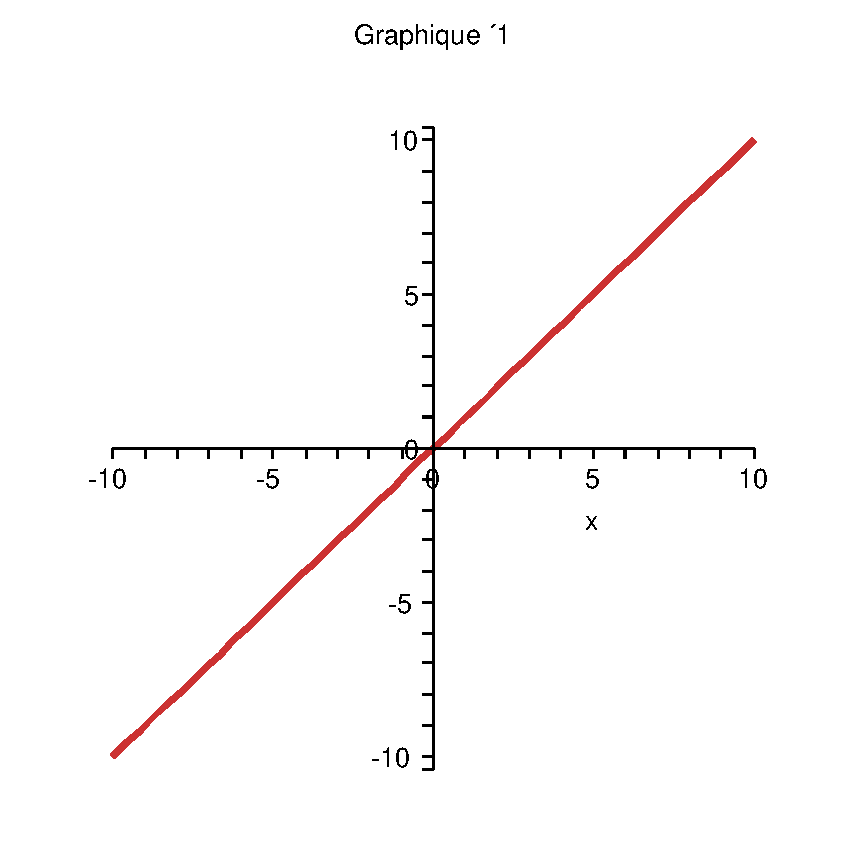
\includegraphics[width=6cm, bb=0 0 400 400]{fonction3.eps}
% fonction3.eps : 300dpi, width=3.39cm, height=3.39cm, bb=0 0 400 400
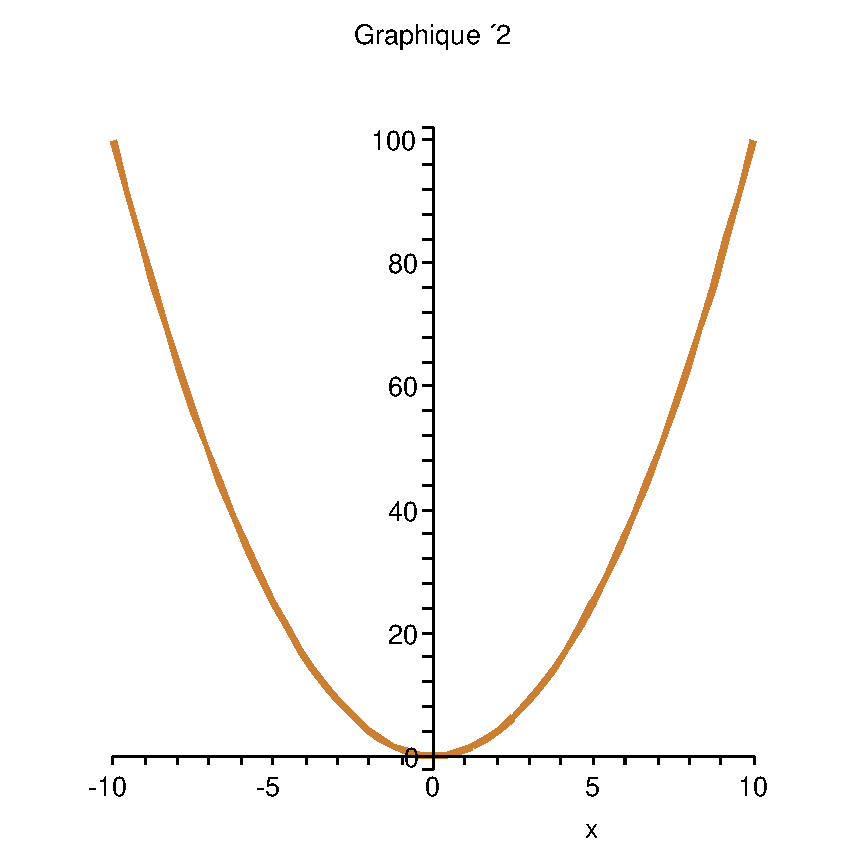
\includegraphics[width=6cm, bb=0 0 400 400]{fonction4.eps}
% fonction4.eps : 300dpi, width=3.39cm, height=3.39cm, bb=0 0 400 400
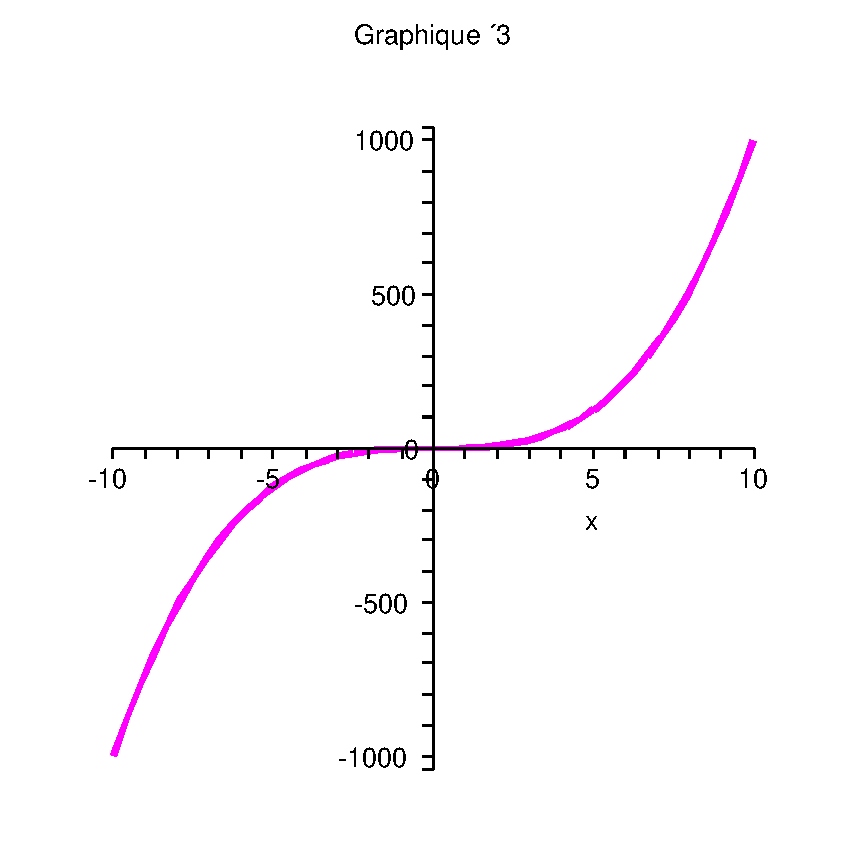
\includegraphics[width=6cm, bb=0 0 400 400]{fonction5.eps}
% fonction5.eps : 300dpi, width=3.39cm, height=3.39cm, bb=0 0 400 400
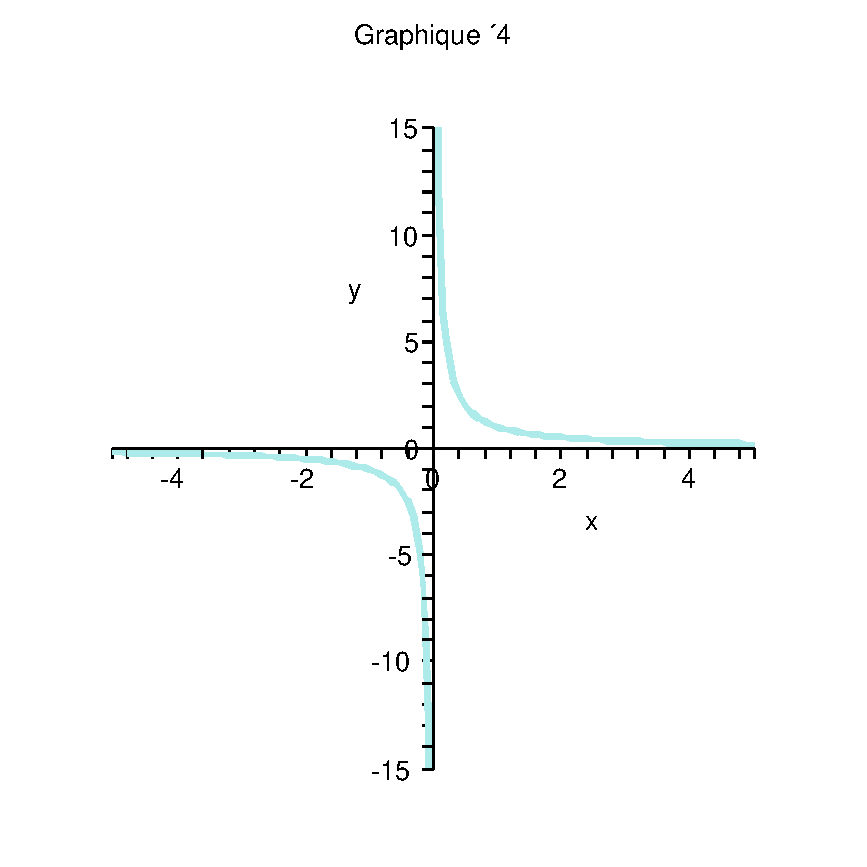
\includegraphics[width=6cm, bb=0 0 400 400]{fonction7.eps}
% fonction7.eps : 300dpi, width=3.39cm, height=3.39cm, bb=0 0 400 400

    \end{center}
a) Plot 1\\
b) Plot 2\\
c) Plot 3\\
d) Plot 4\\

Answer: b)\\

Explanation: \\
Plot 2 represents a second degree polynomial. The correct answer is b).\\

751-- Marc says: ``Mary Jo is my niece``.  Martha answers back:
``You're right but she's not my niece``. Peter asks Mary Jo: ``Is Marc married? `` Mary Jo responds: ``No, but Marc is Martha's brother``.  How is Martha related to Mary Jo? ``\\

a) Martha is Mary Jo's cousin.\\
b) Martha is Mary Jo's grandmother.\\
c) Martha is Mary Jo's mother.\\
d) Martha is Mary Jo's sister.\\
	
Answer: c)\\

Explanation: \\
Since Martha is Marc's sister and not Mary Jo's aunt, Martha is Mary Jo's mother. The correct answer is c).\\

761-- How many cards must Frederick pull out of a normal deck of 52 cards to be sure of having at least 4 black cards?\\

Answer: 30\\

Explanation: \\
If Frederick is very unlucky, the first 26 cards he picks will be red and then the next four will be black. Thus, he must pick 26 + 4 = 30 cards. The correct answer is 30.\\

771-- Aladdin owns a magic lamp whose mass is 1/24 of Aladdin's weight. When he is carrying his lamp he weighs 75\,kg.  What is the mass in kilograms of the magic lamp?\\

Answer: 3\\

Explanation:\\
Let's say\\
$A$ = Aladdin's mass in kilograms; \\
$L$ = Lamp's mass in kilograms.\\

$A\,+\,L=75 \qquad $(equation 1)\\
$24L=A \qquad $ (equation 2)\\

From equation 1 $A$ is replaced with it's value calculated in equation 2.\\
$24L \,+\,L = 75$\\
$25L=75$\\
$L=3$\\
The lamp weighs 3\,kg.\\

781-- Knowing that eight men can dig 8 holes in 32 days. How much time will it take for a man to dig half of a hole.?\\

a) It's impossible.\\
b) 8 days\\
c) 16 days\\
d) 24 days\\

Answer: a)\\

Explanation: \\
It is impossible to dig a half of a hole since half of a hole is in fact a hole! The correct answer is a).\\

791-- A caterpillar takes off on a long voyage. It must climb up a 12 m brick wall to reach its destination. The caterpillar climbs 4 m during the day and falls 2 m during the night.  If it starts its ascent today, how many whole days will it take to reach the wall's summit?\\

a) 3 days\\
b) 4 days\\
c) 5 days\\
d) 6 days\\

Answer: b)\\

Explanation: \\

\begin{tabular}{|c|c|c|} \hline
{\bf Morning} & {\bf Number of days traveled} & {\bf Height in meters} \\
\hline \hline

1 & 0 & 0 \\ \hline
2 & 1 & 2\\ \hline
3 & 2 & 4\\ \hline
4 & 3 & 6\\ \hline
5 & 4 & 8\\ \hline
\multicolumn{3}{c}{}\\

\end{tabular}\\

After four days of travelling, the caterpillar has reached a heigth of 8 m. During the fifth day, it climbs four more meters and reaches the top or 12 m high.  Thus, the caterpillar must travel for 4 entire days to reach the wall's summit.
The correct answer is b).\\

801-- Philo wants to meet up with his girlfriend Sophie, but he doesn't want to be accompanied by his other friends. So, he gives Sophie a code card from which she can read $13\,-\,15\,-\,22\,-\,9\,-\,5\,-\,20\,-8\,-5\,-1\,-20\,-5\,-18$.
Where should Sophie go to meet up with Philo?\\

Answer: To the movie theater\\

Explanation: \\
Each letter has been replaced by its corresponding number. \\
a = 1\\
b = 2\\
c = 3\\
d = 4\\
e = 5\\
$\vdots$\\
z = 26\\

We thus have\\
13 = m\\
15 = o\\
22 = v\\
9 = i\\
5 = e\\
20 = t\\
8 = h\\
5 = e\\
1 = a\\
20 = t\\
5 = e\\
18 = r.\\

The correct answer is movie theater.\\

811-- Mathcity's day camp has a certain number of teenagers aged between 12-14 years old. Camp counselors can choose between creating groups of 2, 3, 4, or 6 people and in each case, no child is left by itself.  Knowing that there are between 25 and 40 kids between 12 and 14 years old, what is the total amount of kids at day camp?\\

Answer: 36\\

Explanation: \\
$36=2\times18=3\times12=4\times9=6\times6$\\
The correct answer is 36.\\

821-- What are the chances of winning the Lotto 6/49?\\
a) $\frac{1}{13\,983\,816}$\\ [2mm] b) $\frac{1}{1\,023\,245}$\\
[2mm] c) $\frac{6}{49}$\\ [2mm]
d) $\frac{49}{6}$\\

Answer: a)\\

Explanation: \\
To win the Lotto 6/49 jackpot, one must correctly select 6 numbers out of 49. The number of possibilities in choosing 6 numbers out of 49 is determined by the following calculation:\\[2mm]
$\frac{49!}{\left( 49\,-\,6\right)
!\,6!}=\frac{49!}{43!\,6!}=\frac{44\cdot45\cdot46\cdot47\cdot48\cdot49}{1\cdot2\cdot3\cdot4\cdot5\cdot6}=13\,983\,816$.\\[2mm]
There is a one out of $13\,983\,816$ chance of winning the Lotto 6/49. The correct answer is a).\\

831-- In the message ``YMLUPLTI HETER TSMIE RFUO`` the letters in in each word were mixed up. However, each word is in the correct order. What should the answer to the message be?\\
a) 10\\
b) 12\\
c) 14\\
d)  16\\

Answer: b)\\

Explanation: \\
The message is: ``MULTIPLY THREE TIMES FOUR``.\\
$3\times4=12$\\
The correct answer is b).\\

841-- A domino is formed from two squares of the same size with each square touching another square with one side. Placing three squares side by side forms a trimino, while placing five squares side by side forms a pentamino.  How many different pentaminos are there?\\

a) 5\\
b) 8\\
c) 12\\
d) 15\\

Answer: c)\\

Explanation: \\
There are 12 different pentaminos.  The correct answer is c).\\

851-- Smith and Smythe are in a session of truth and lies. Mondays, Wednesdays and Fridays Smith lies; on every other day he tells the truth. Tuesdays, Thursdays, Saturdays and Sundays Smythe lies; and on the other days he tells the truth. Today, Smith and Smythe both say: ``Yesterday, I told the truth.``  What day is it?\\


Answer: Sunday\\

Explanation: \\

\begin{tabular}{|c|c|c|} \hline
{\bf Day} & {\bf Smith} & {\bf Smythe} \\ \hline \hline

Monday    & Lies  &  Tells the truth      \\ \hline
Tuesday   & Tells the truth      &  Lies  \\ \hline
Wednesday & Lies  &  Tells the truth      \\ \hline
Thursday  & Tells the truth      &  Lies  \\ \hline
Friday    & Lies  &  Tells the truth      \\ \hline
Saturday  & Tells the truth      &  Lies  \\ \hline
Sunday    & Tells the truth  &  Lies      \\ \hline
\multicolumn{3}{c}{}\\
\end{tabular}\\

\begin{tabular}{|c|c|c|} \hline
{\bf Day} & {\bf What Smith says } & {\bf What Smythe says } \\ \hline
\hline

Monday     & Yesterday, I lied.       &  Yesterday, I told the truth.   \\ \hline
Tuesday     & Yesterday, I lied.      &  Yesterday, I lied.       \\
\hline Wednesday  & Yesterday, I lied.      &  Yesterday, I lied.
\\ \hline Thursday     & Yesterday, I lied.      &  Yesterday, I lied.
\\ \hline Friday  & Yesterday, I lied.      &  Yesterday, I lied.
\\ \hline Saturday    & Yesterday, I lied.      &  Yesterday, I lied.
\\ \hline Sunday  & Yesterday, I told the truth.  &  Yesterday, I told the truth.       \\ \hline
\end{tabular}\\

The correct answer is Sunday.  \\

861-- How many different and discernable arrangements can be made with the letters in the word \sloppy \mbox{COMBINATION?}\\

a) $4\,989\,600$\\
b) $9\,979\,200$\\
c) $19\,958\,400$\\
d) $39\,916\,800$\\

Answer: a)\\

Explanation: \\
The word COMBINATION contains 11 letters, 8 of which are not the same. N, I and O are each repeated twice.\\
If each letter was different in the word, there would be
$11!\,=11\times10\times9\times8\times7\times6\times5\times4\times3\times2\times1=39\,916\,800$
arrangements.  However, the two N's, two I's and two O's are not detectable, thus diminishing the number of arrangements. Therefore, there are
$\frac{11!}{2!\,2!\,2!}=\frac{11\times10\times9\times8\times7\times6\times5\times4\times3\times2\times1}{2\times1\times2\times1\times2\times1}=4\,989\,600$
different arrangements. The correct answer is a).\\

871-- Three of the following results are attributed to Thales of Miletos and Pythagoras. Which one is attributed to Pythagoras?\\

a$)$ The angles at the base of an isoceles triangle are congruent.\\
b$)$ A good approximation of the irrational number $\sqrt2$ \\
c$)$ The case of congruency of angle-side-angle triangles \\
d$)$ A line parallel to a side of a triangle drawn from one side to the other divides both sides in a proportionate fashion.\\

Answer: b$)$\\

Explanation: \\
The results \og The angles at the base of an isoceles triangle are congruent\fg , \og the case of congruency of angle-side-angle triangles\fg\ and  \og a parallel line drawn to one side of a triangle divides the other two sides in a proportionate fashion\fg\ are all attributed to Thales of Miletos. On another note, it is important to recognize that even if the result \og one parallel line drawn through one side of a triangle divides the other two sides in a proportionate manner\fg\ is attributed to Thales of Miletos, we ignore who truly discovered this result. Pythagoras is credited with the first good approximation of $\sqrt2$. The correct answer is b$)$.

        \begin{center}
        Pythagore\\
    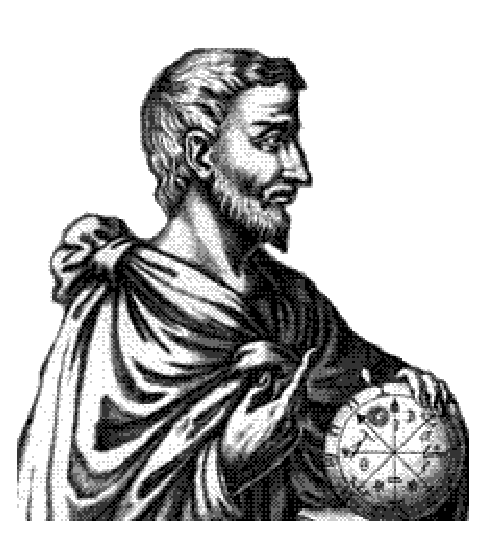
\includegraphics[width=6cm]{pythagore1.eps}\\
        {\footnotesize http
://www.univ-ouaga.bf/laboratoires/lame/images/pythagore/pythagore1.gif}
    \end{center}

881-- Which of the following mathematicians lived in the 5th century B.C.?\\

a$)$ Franciscus Vieta \\
b$)$ Galileo Galilei \\
c$)$ Hippocrates of Chios \\
d$)$ Pietro Cataldi\\

Answer: c$)$\\

Explanation: \\
Hippocrates of Chios was born in 470 B.C., Franciscus Vieta in 1540, Pietro Cataldi in 1548 and Galileo Galilei in 1564. Thus, the correct answer is c$)$.\\

        \begin{center}
        Hippocrate de Chios\\
    
\includegraphics[width=6cm]{Hippocrates.eps}\\
        {\footnotesize http
://www.answers.com/main/content/wp/en/thumb/3/32/240px-Hippocrates.jpg}
    \end{center}

891-- Three of the following subjects were mentioned in Euclid's Elements. The last subject was only studied after Christ by Nicholas Oresme. What was this subject?\\
	
a$)$ Fractional exponents \\
b$)$ Geometric Algebra \\
c$)$ Solid Geometry \\
d$)$ Irrational numbers\\

Answer: a$)$\\

Explanation: \\
Fractional exponents was a subject studied after Christ by a man named Nicholas Oresme. The correct answer is a$)$.\\

        \begin{center}
        Nicholas Oresme\\
    
\includegraphics[width=6cm]{oresme.eps}\\
        {\footnotesize http
://www.math-inf.uni-greifswald.de/mathematik+kunst/pic/objekte/oresme-200.jpg}
    \end{center}

901-- Which Roman general ordered the drawing of a geometric configuration on Archimedes' tombstone?\\

a$)$ Augustus \\
b$)$ Julius Caesar \\
c$)$ Marcellus \\
d$)$ Tiberius \\

Answer: c$)$\\

Explanation: \\
Marcellus had a lot of respect for Archimedes. The correct answer is c$)$.\\

        \begin{center}
        Archimedes of Syracuse\\
    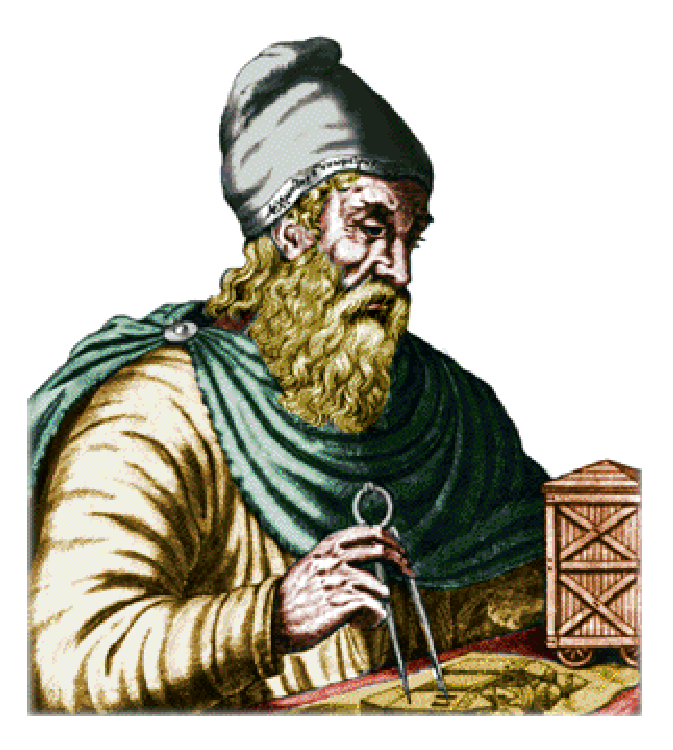
\includegraphics[width=6cm]{archimede.eps}\\
        {\footnotesize http
://www.cattolica.info/cultura/fisica/biblioteca/personaggi/images/archimede.gif}
    \end{center}

911-- During which century did Archimedes of Syracuse, Eratosthenes and Apollonius of Perga live?\\

a$)$ 10th Century \\
b$)$ 3rd Century \\
c$)$ 3rd Century B.C. \\
d$)$ 20th Century   \\

Answer: c$)$\\

Explanation: \\
Archimedes of Syracuse lived from 287-212 B.C., Eratosthenes from 276-190 B.C. and Apollonius of Perga from 262-190 B.C. Thus, they lived in the 3rd Century B.C. The correct answer is c$)$.\\

921-How did al Khwarizmi become famous during his time period?\\

a$)$ By discovering dinosaur bones \\
b$)$ By discovering irrational numbers \\
c$)$ By observing the circular movement of planets \\
d$)$ By creating astronomical tables \\

Answer: d$)$\\

Explanation: \\
Al Khwarizmi became famous for creating astronomy tables.
The correct answer is d$)$.\\

931-In which of the following professions did Omar Khayyam excel?\\

a$)$ Professional hockey player \\
b$)$ Painter \\
c$)$ Poet \\
d$)$ Sculptor \\

Answer: c$)$\\

Explanation: \\
Omar Khayyam was one of the greatest Persian poets. The correct answer is c$)$.\\

        \begin{center}
        Omar Khayyam\\
    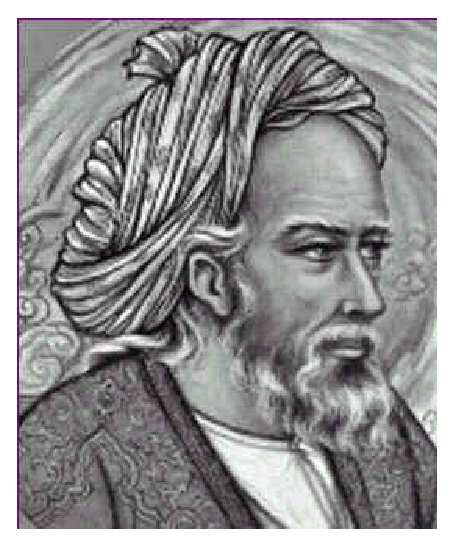
\includegraphics[width=6cm]{Omar.eps}\\
        {\footnotesize http
://www.shunya.net/Text/Islam/Maps/OmarKhayyam.jpg}
    \end{center}


951- During a certain time period mathematicians were also very interested in other sciences. Which mathematician was the first to observe the circular movement of the planets?\\

a$)$ Alan Baker \\
b$)$ George Darwin \\
c$)$ Nicolas Bourbaki  \\
d$)$ Nicholas Copernicus \\

Answer: d$)$\\

Explanation: \\
Nicholas Copernicus was the first to observe the circular movement of the planets. However, he didn't publish his works until a few days before he died because he feared receiving negative reactions from other theologists from that time period. His fears became legitimate as in 1616, Pope Paul V condemned the advanced ideas of Copernicus as being contrary to the "Writings". Thus, the correct answer is d$)$.\\

        \begin{center}
        Nicholas Copernicus\\
    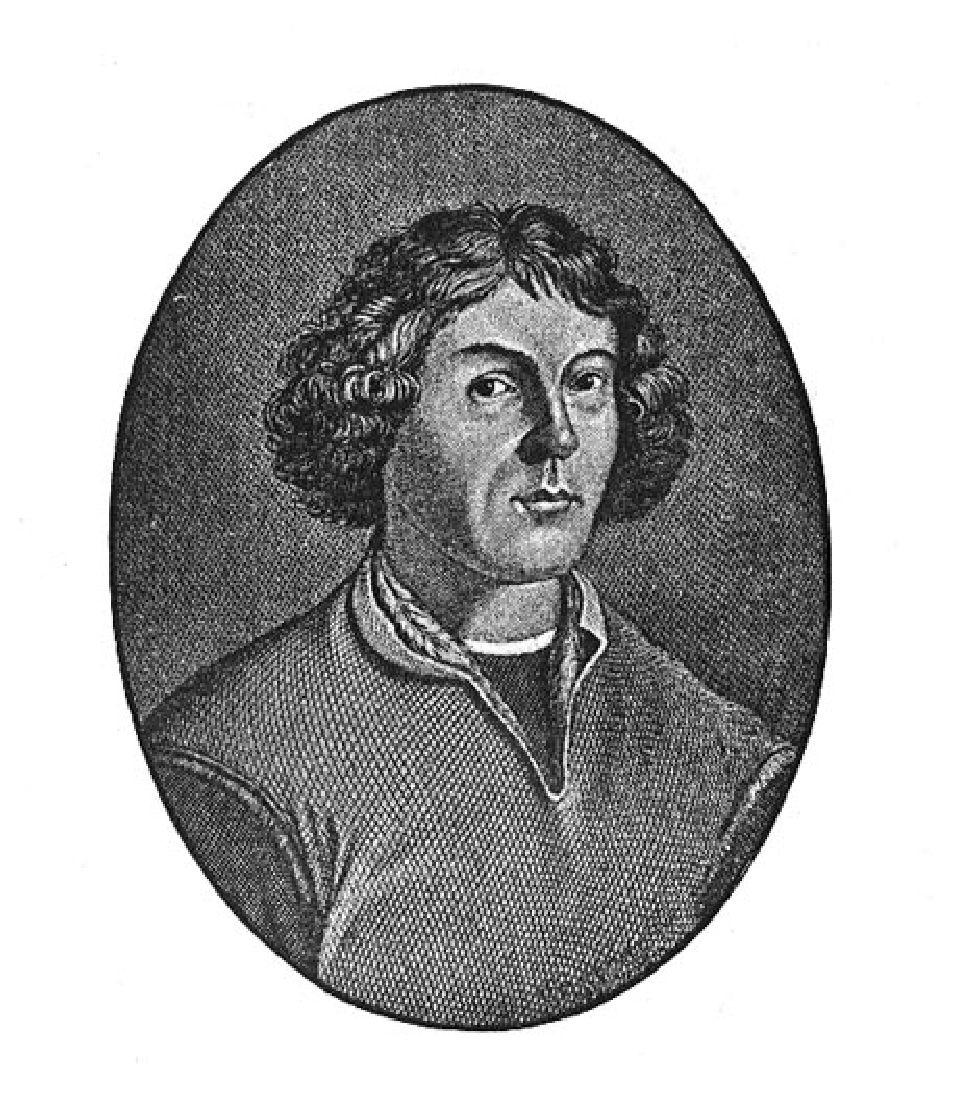
\includegraphics[width=6cm]{Copernic.eps}\\
        {\footnotesize http ://www.asso-copernic.org/images/Copernic.jpg}
    \end{center}

961- One day, Jerome Cardan found out that Tartaglia had discovered the solution to the cubic equation. He then began to continuously praise Tartaglia and eventually convinced him to reveal his method while promising under oath never to publish his work before Tartaglia had a chance to do it. Why did Cardan end up publishing Tartaglia's results?\\

a$)$ Because del Ferro had also discovered the method. \\
b$)$ Because Tartaglia had died.  \\
c$)$ Because Tartaglia had finally given him permission to do so.  \\
d$)$ Because he had gotten into an argument with Tartaglia. \\

Answer: a$)$\\

Explanation: \\
Cardan published the results because del Ferro had also discovered the method and had entrusted it on his deathbed to his student Antonio Fiore. When Cardan was informed of this disclosure, he felt free from his promise and then went on to publish his work {\sl Ars Magna}, to the great dismay of Tartaglia. The correct answer is a$)$.\\

        \begin{center}
        Gerolamo Cardano\\
    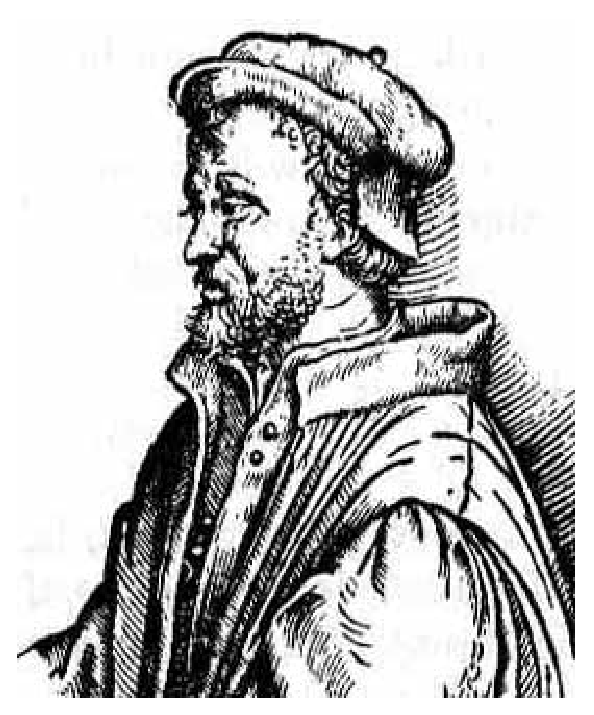
\includegraphics[width=6cm]{Cardan.eps}\\
        {\footnotesize http ://www.mathematik.ch/mathematiker/Cardan.jpg}
    \end{center}

        \begin{center}
        Nicc\`olo Fontana\\
    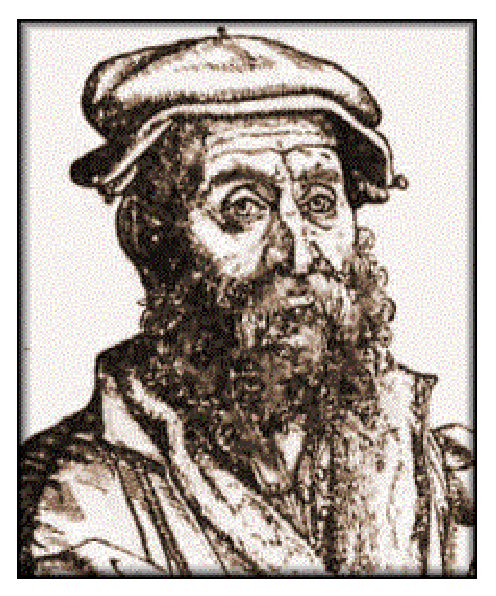
\includegraphics[width=6cm]{Tartaglia.eps}\\
        {\footnotesize http
://perso.wanadoo.fr/frederic.gales/Tartaglia.gif}
    \end{center}

971-During which century did mathematicians Jerome Cardan, Robert Recorde, Lodovico Ferrari and Raphael Bombelli all live?\\

a$)$ Second Century B.C.\\
b$)$ 19th Century \\
c$)$ 16th Century  \\
d$)$ 3rd Century \\

Answer: c$)$\\

Explanation: \\
These mathematicians all lived in the 16th Century. The correct answer is c$)$.\\

981-At the beginning of Henry IV's reign, what was Philippe II, the King of Spain, complaining about to the Pope?\\

a$)$ About Fran\c cois Vi\`ete being a thief. \\
b$)$ About Fran\c cois Vi\`ete performing magical practices contrary to the Christian faith. \\
c$)$ About Fran\c cois Vi\`ete not being a true Frenchman. \\
d$)$ About Fran\c cois Vi\`ete's results being contradictory to religion. \\

Answer: b$)$\\

Explanation: \\
The King was complaining that Fran\c cois Vi\`ete's magical practices were contrary to the Christian faith. Philippe II made a complaint because Vi\`ete was extremely effective in decoding Spain's secret messages when Henry IV was fighting against the Spanish allies, the Line.  The correct answer is b$)$.\\

        \begin{center}
        Fran\c cois Vi\`ete\\
    
\includegraphics[width=6cm]{viete.eps}\\
        {\footnotesize http ://www.antiqua.altervista.org/viete.jpg}
    \end{center}

        \begin{center}
        Philippe II\\
    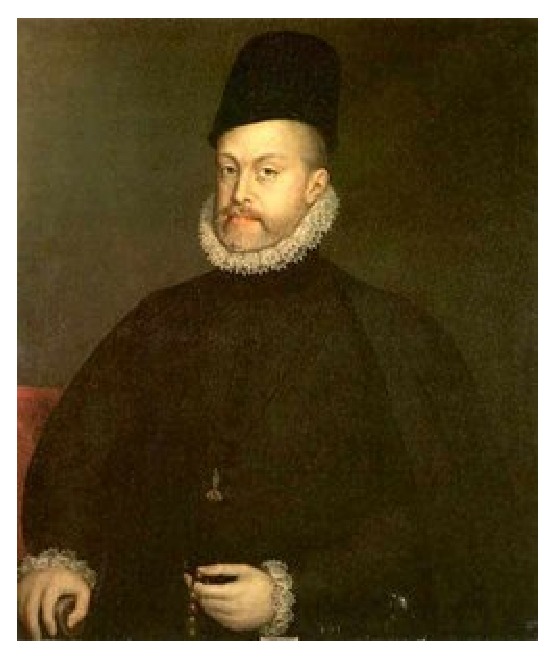
\includegraphics[width=6cm]{phil.eps}\\
        {\footnotesize http
://upload.wikimedia.org/wikipedia/fr/thumb/c/c1/250px-Philippe\_II\_espagne.jpg}
    \end{center}

        \begin{center}
        Henri IV\\
    
\includegraphics[width=6cm]{henri.eps}\\
        {\footnotesize http
://www.uqac.uquebec.ca/zone30/Classiques\_des\_sciences\_sociales\\
        /classiques/henri\_iv/henri\_iv\_photo/henri\_iv\_larousse\_50.gif}
    \end{center}

991-Which of the following inventions is accredited to Johannes Kepler?\\

a$)$ The Roberval balance \\
b$)$ The pendulum clock \\
c$)$ The Keplerian telescope \\
d$)$ The reflecting telescope\\

Answer: c$)$\\

Explanation: \\
The Keplerian telescope was invented by Johannes Kepler.
The correct answer is c$)$.\\

        \begin{center}
        Johannes Kepler\\
    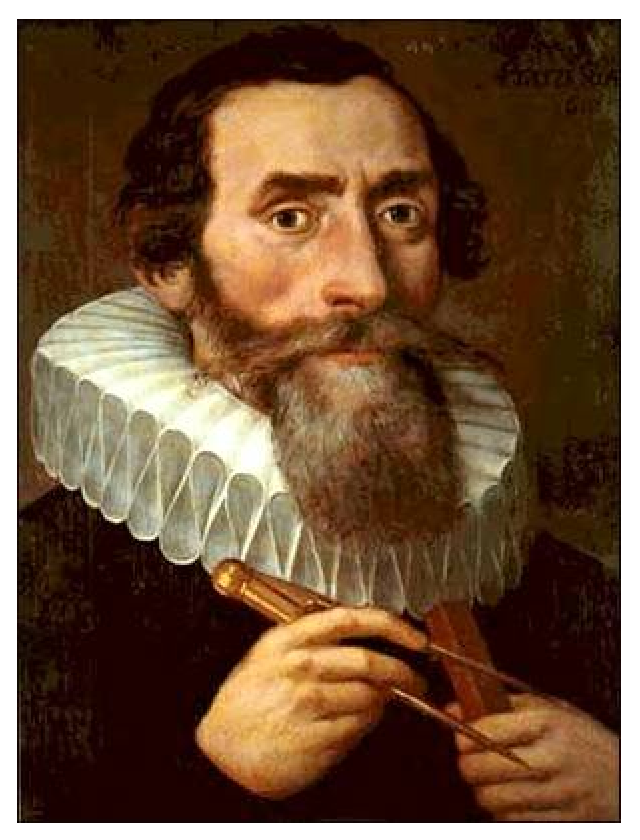
\includegraphics[width=6cm]{kepler.eps}\\
        {\footnotesize http ://www.spacefame.org/kepler.jpg}
    \end{center}




\end{document}
